Os parâmetros estimados em um sistema dinâmico estão sujeitos à incerteza presente na captura dos dados, tal como erros de mensuração ou a variabilidade natural dos dados, e nas hipóteses adotadas pelo método de estimação. 
Assim, nessa seção, o objetivo será construir intervalos de confiança para os parâmetros desconhecidos de forma que, no longo prazo, a proporção dos intervalos calculados que contêm o parâmetro seja o nível desejado. 
Utilizaremos o {\em método Bootstrap} \cite{efron1986} que tem uma abordagem por simulação baseada nos dados. Ele gera, a partir de uma série $Y$, dados replicados $Y_1^*, ...., Y_N^*$ e realiza as estimações para cada um. 
Os intervalos de confiança para os valores de interesse são, então, os percentis correspondentes das $N$ amostras replicadas \cite{joshi2006}. 

Como consequência da estrutura dos erros apresentada nas equações \eqref{obsT1} e \eqref{obsD1}, as curvas são geradas com o valor inicial $\hat{T}(0) = y_0^{(1)}$ e para cada $i \ge 1$, $\hat{T}(i+1) = \hat{T}(i) + \varepsilon_{i+1}$, em que $\varepsilon_{i+1} \sim \mathcal{N}(\hat{x}_{i+1}^{1}, \hat{\sigma}_1^2)$ e $\hat{\sigma}_1^2$ é a estimativa para $\sigma_1^2$. A construção é análoga para a curva de óbitos.
Os parâmetros, então, foram estimados para cada uma das simulações. 
Além disso, para evitar que todas as simulações resultem em uma mesma região com mínimo locais, aleatorizamos o chute inicial do algoritmo de otimização. Para cada $j$ entre $1$ e $r+s+1$, $\theta_j^{inicial}$ é tomado aleatoriamente com distribuição uniforme no intervalo $(l_j, u_j)$, isto é, entre os limites inferior e superior estabelecidos. Realizamos esse processo $m$ vezes e tomamos a estimação com menor erro na função objetivo (equação \eqref{objective}). 

Fizemos $N = 500$ simulações com $m = 10$ (ou seja, $5000$ simulações no
total) e os outros parâmetros definidos como na Seção \ref{residual-analysis}. Após as simulações, estimamos os intervalos de confiança para os
parâmetros com nível 95\%, assim como as curvas $\mathcal{R}_t$ induzidas a
cada tempo $t$. O intervalo estimado para a taxa de subnotificação $\alpha$
foi $(0.849,0.931)$. Na Figura \ref{fig:rt-confidence-interval}, é possível
visualizar os intervalos de $\mathcal{R}_t$. É interessante visualizar o
gráfico que exibe as relações dois a dois entre os parâmetros, o que mostra a
correlação nas estimações. 
As correlações estimadas na Figura \ref{fig:corr-matrix} podem ser observadas
nos gráficos de dispersão na Figura \ref{fig:correlation-bootstrap}, como, por
exemplo, a relação linear entre $\alpha$ e $\beta_2$. 
Os histogramas dos parâmetros também podem ser observados. Na Tabela \ref{tab:bootstrap-estimations} é sumarizada a informação para todos os parâmetros. Informações e gráficos adicionais podem ser visualizados no Github \cite{github}.

\begin{figure}
    \centering
    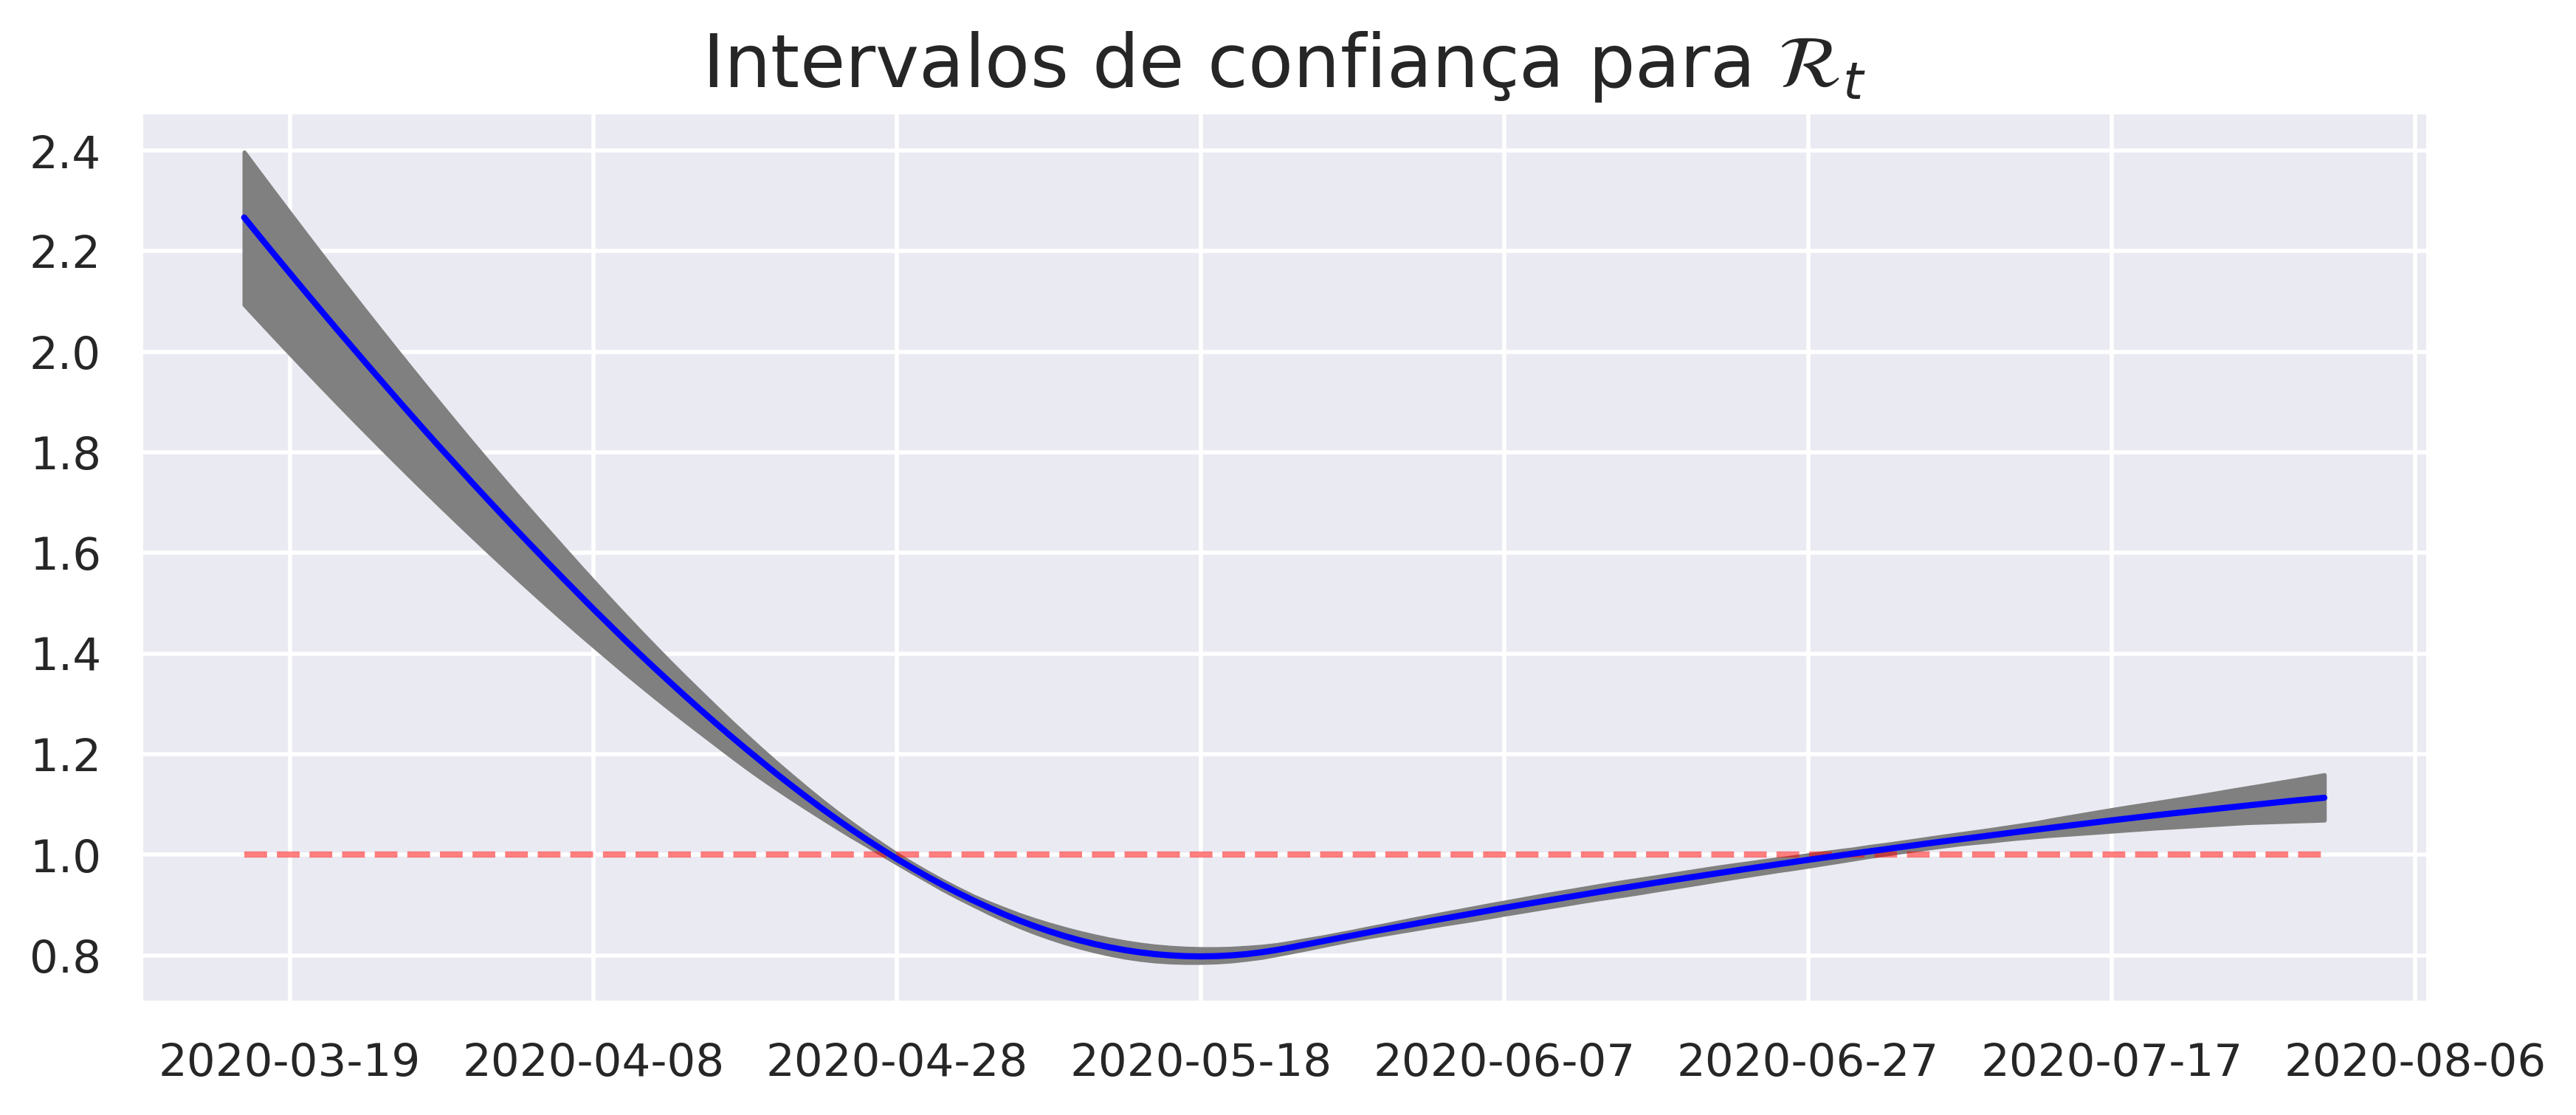
\includegraphics[width = 0.9\textwidth]{../images/rt_confidence_interval.png}
    \caption{A curva em azul é a mediana das curvas estimadas e em cinza o
    intervalo de confiança. Em vermelho é o limiar 1 para o $\mathcal{R}_t$.}
    \label{fig:rt-confidence-interval}
\end{figure}

\begin{figure}
    \centering
    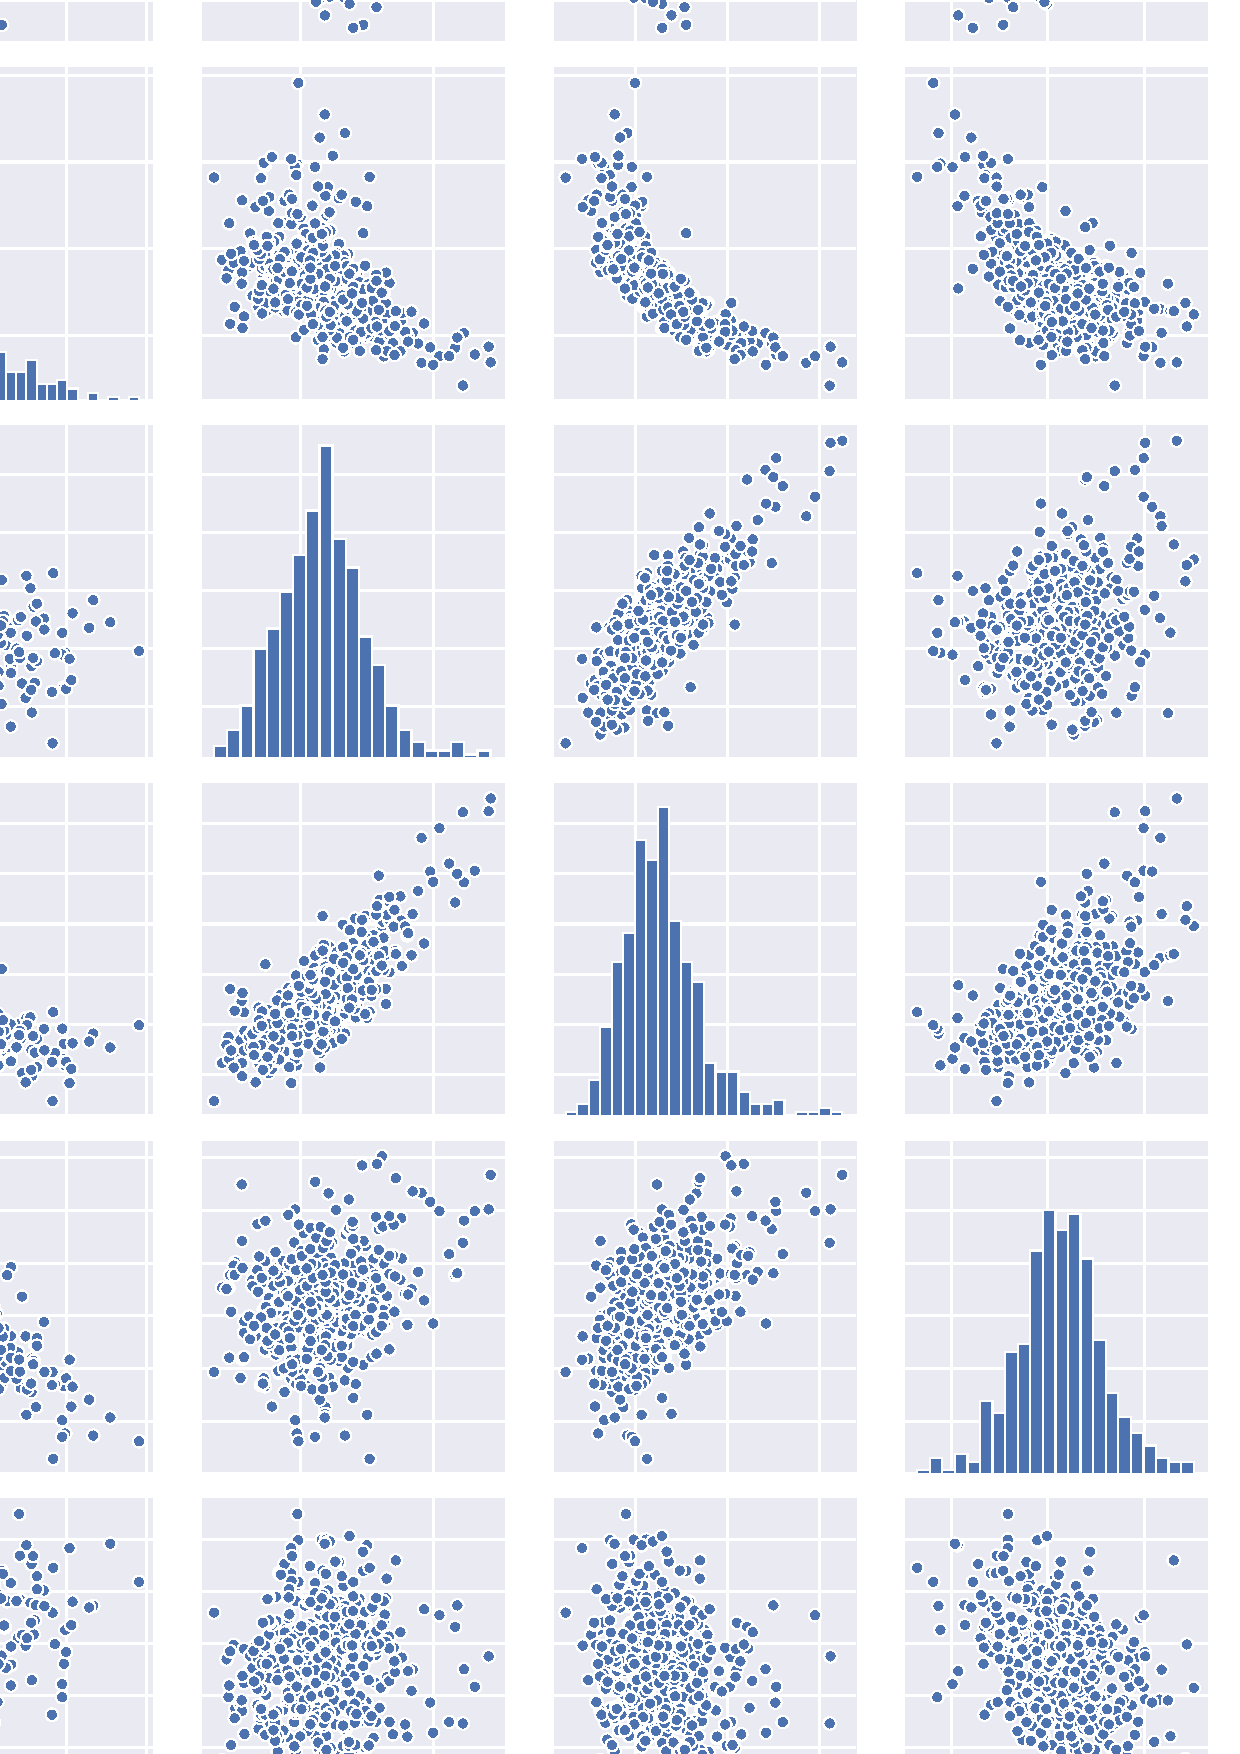
\includegraphics[width = \textwidth]{../images/correlation_bootstrap.png}
    \caption{Gráficos de dispersão a cada dois parâmetros indicando a relação entre eles e os histogramas das estimativas.}
    \label{fig:correlation-bootstrap}
\end{figure}

\begin{table}[!ht]
    \centering
    \begin{tabular}{|c|c|c|}
    \hline
    \textbf{Parâmetro} & \textbf{Mediana} & \textbf{Intervalo calculado} \\ \hline
    $\alpha$        & $0.903$            & $[0.849,0.93]$                      \\ \hline
    $\beta_1$      & $0.144$          & $[0.142, 0.147]$                        \\ \hline
    $\beta_2$      & $0.073$          & $[0.069, 0.079]$                        \\ \hline
    $\beta_3$      & $0.101$          & $[0.098, 0.104]$                        \\ \hline
    $\beta_4$      & $0.126$          & $[0.123, 0.132]$                        \\ \hline
    $\mu_1$    & $0.0101$        & $[0.0092, 0.011]$                       
    \\ \hline
    $\mu_2$    & $0.0159$        & $[0.0154, 0.0164]$               
    \\ \hline
    $\mu_3$    & $0.0103$        & $[0.0098, 0.0108]$                       
    \\ \hline
    $\mu_4$    & $7.03\cdot 10^{-3}$        & $[6.73\cdot 10^{-3}, 7.38\cdot 10^{-3}]$                       
    \\ \hline
    \end{tabular}
    \caption{Estimativas da mediana e dos intervalos de confiança para cada parâmetro desconhecido do modelo.}
    \label{tab:bootstrap-estimations}
\end{table}